\chapter{Numbers 17}

\begin{figure}
  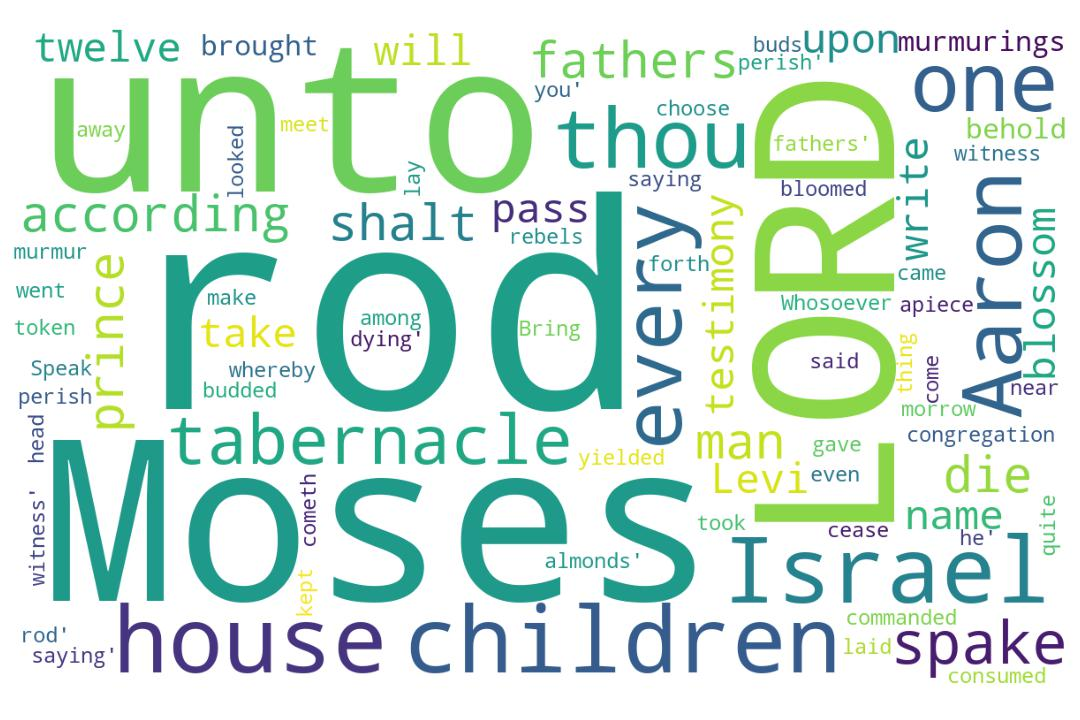
\includegraphics[width=\linewidth]{04OT-Numbers/Numbers17-WordCloud.jpg}
  \caption{Numbers 17 Word Cloud}
  \label{fig:Numbers 17 word Cloud}
\end{figure}

\marginpar{\scriptsize \centering \fcolorbox{bone}{lime}{\textbf{SHHHH}}\\ (Numbers 17:1-13) \begin{compactenum}[I.][8]
    \item  \textbf{Placement} \index[scripture]{Numbers!Num 17:04} (Numbers 17:4) 
    \item  \textbf{Purpose} \index[scripture]{Numbers!Num 17:05} (Numbers 17:5) 
    \item  \textbf{Princes} \index[scripture]{Numbers!Num 17:06} (Numbers 17:6) 
    \item  \textbf{Presence} \index[scripture]{Numbers!Num 17:07} (Numbers 17:7) 
    \item  \textbf{Prevention} \index[scripture]{Numbers!Num 17:10} (Numbers 17:10) 
    \item  \textbf{Perishing} \index[scripture]{Numbers!Num 17:12} (Numbers 17:12) 
    \item  \textbf{Pruning} %\index[scripture]{Numbers!Num 17:12} (Numbers 17:12) 
\end{compactenum}}
    



\footnote{\textcolor[cmyk]{0.99998,1,0,0}{\hyperlink{TOC}{Return to end of Table of Contents.}}}\footnote{\href{https://audiobible.com/bible/numbers_17.html}{\textcolor[cmyk]{0.99998,1,0,0}{Numbers 17 Audio}}}\textcolor[cmyk]{0.99998,1,0,0}{And the LORD spake unto Moses, saying,}
[2] \textcolor[cmyk]{0.99998,1,0,0}{Speak unto the children of Israel, and take of every one of them a rod according to the house of \emph{their} fathers, of all their princes according to the house of their fathers twelve rods: write thou every man's name upon his rod.}
[3] \textcolor[cmyk]{0.99998,1,0,0}{And thou shalt write Aaron's name upon the rod of Levi: for one rod \emph{shall} \emph{be} for the head of the house of their fathers.}
[4] \textcolor[cmyk]{0.99998,1,0,0}{And thou shalt lay them up \fcolorbox{bone}{lime}{in the tabernacle} of the congregation before the testimony, where I will meet with you.}
[5] \textcolor[cmyk]{0.99998,1,0,0}{And it shall come to pass, \emph{that} the man's rod, whom I shall choose, \fcolorbox{bone}{lime}{shall blossom}: and I will make to cease from me the murmurings of the children of Israel, whereby they murmur against you.}\\
\\
\P \textcolor[cmyk]{0.99998,1,0,0}{And Moses spake unto the children of Israel, and every one of their \fcolorbox{bone}{lime}{princes} gave him a rod apiece, for each prince one, according to their fathers' houses, \emph{even} twelve rods: and the rod of Aaron \emph{was} among their rods.}
[7] \textcolor[cmyk]{0.99998,1,0,0}{And Moses laid up the rods \fcolorbox{bone}{lime}{before the LORD} in the tabernacle of witness.}
[8] \textcolor[cmyk]{0.99998,1,0,0}{And it came to pass, that on the morrow Moses went into the tabernacle of witness; and, behold, the rod of Aaron for the house of Levi was budded, and brought forth buds, and bloomed blossoms, and yielded almonds.}\footnote{\textbf{Hebrews 9:4} - Which had the golden censer, and the ark of the covenant overlaid round about with gold, wherein was the golden pot that had manna, and Aaron’s rod that budded, and the tables of the covenant;}
[9] \textcolor[cmyk]{0.99998,1,0,0}{And Moses brought out all the rods from before the LORD unto all the children of Israel: and they looked, and took every man his rod.}\\
\\
\P \textcolor[cmyk]{0.99998,1,0,0}{And the LORD said unto Moses, Bring Aaron's rod again before the testimony, to be kept for a token \fcolorbox{bone}{lime}{against the rebels}; and thou shalt quite take away their murmurings from me, that they die not.}
[11] \textcolor[cmyk]{0.99998,1,0,0}{And Moses did \emph{so}: as the LORD commanded him, so did he.}
[12] \textcolor[cmyk]{0.99998,1,0,0}{And the children of Israel spake unto Moses, saying, Behold, we die, we \fcolorbox{bone}{lime}{perish}, we all perish.}
[13] \textcolor[cmyk]{0.99998,1,0,0}{Whosoever cometh any thing near unto the tabernacle of the LORD shall die: shall we be consumed with dying?}